\documentclass{beamer}
\usepackage[utf8]{inputenc}
\usepackage{xeCJK}
\setCJKsansfont{SimSun}
\usepackage{graphics}
\usepackage{ctex} 
\usepackage{subfigure}
\usepackage{listings}
\usepackage{xcolor}
\usepackage{bookman}
\usepackage{xspace}
\usepackage{caption}



\usetheme{Madrid}
\usecolortheme{default}

%-------------------------------------------

\title[|网络科学导论|] %optional
{Collective patterns of social diffusion are shaped by individual inertia and trend-seeking}

\subtitle{『集体的社会扩散模式由个体的惯性和趋向性决定』}

\author[授课老师:梁海丽] % (optional)
{~}
\institute[SHU] % (optional)
{
	\Large{
		\begin{block}{\centerline{Shanghai University}}
	\centerline{\large{Jie Xing}-\normalsize{20121192@ICS}\\}
	\centerline{\large{Shiwei Wang}-\normalsize{20121016@Automation}\\}
	\centerline{\large{Sicheng Zhang}-\normalsize{19123001@Industrial Engineering}\\}
        \end{block}}
	%\and
}

\date[2022-11-03] % (optional)
{Nov.03, 2022}

\logo{
\includegraphics[height=1.3cm]{SHU.pdf}}


%------------------------------------------------------------

\AtBeginSection[]
{
	\begin{frame}
		\frametitle{Contents}
		\tableofcontents[currentsection]
	\end{frame}
}
%------------------------------------------------------------

\begin{document}
	
	%The next statement creates the title page.
	\frame{\titlepage}
	
	
	%---------------------------------------------------------

	\begin{frame}
		\frametitle{Contents}
		\tableofcontents
	\end{frame}

%---------------------------------------------------------

\section{Introduction}
\begin{frame}
	\sectionpage
\end{frame}
	\begin{frame}{Some Concepts}

		
\begin{block}{社会扩散}<1-> 
	当个人共同采用一种替代方案改变现状,造成社会习俗发生改变,这一过程称为社会扩散。
\end{block}

\begin{block}{社会习俗}<2-> 
	社会和文化的基本方面,如握手、鞠躬或公认的语法规则和词义等。
\end{block}

\begin{block}{探索者与非探索者}<3-> 
	社会扩散过程中,每个人扮演不同的角色。未提出承诺的一小部分人会首先测试替代方案,
	他们常常会多次转换策略,称之为\textbf{探索者},可能引起向其他人口快速扩散,从现状转变策略,
	这部分人称之为\textbf{非探索者}。
\end{block}

	\end{frame}


\begin{frame}{Some Concepts}
		\begin{block}{Bass模型}
			Bass模型最早是由美国的Frank Bass提出来的,最开始是一个用来预测耐用消费品销售情况的模型。
			该模型的基本假设是顾客的最初购买时间和以前购买者的数目相关,它的三个基本参数是:外部影响系数p、
			内部影响系数q、市场潜力m,可以用历史数据来预测销售高峰。
		\end{block}
		\begin{block}{}
		\begin{equation*}
			\begin{aligned}
				\frac{\mathrm{d} N(t)}{\mathrm{d} t}=p[m-N(t)]+q\frac{N(t)}{m}[m-N(t)]
			\end{aligned}
		\end{equation*}
	    \end{block}
\end{frame}


\begin{frame}{Some Concepts}
	\begin{itemize}
	\item ABM模型
	 \begin{itemize}
		%首先,来了解一下ABM模型。
		\item<1->  ABM是计算机模拟的一种,译为代理人基模型,又称多元代理人系统或多智能体系统,
		是一种用来模拟具有自主意识的智能体(独立个体或共同群体,例如组织、团队)的行动和相互作用的计算模型,通过图像展示和评估智能体在系统整体中的作用。ABM也综合了一些其他思想,比如博弈论、复杂系统、涌现、计算社会学、多智能体系统和演化计算等。
		\item<2->  一个ABM模型主要包括以下要素 :一定数量的“代理人” ;一定数量的“代理人”之间的关系;一个模拟“代理人”的行为和互动的框架。ABM明确了模拟个体或对象的行为在时间和空间中的因果关系。
		%从概念上来说,在ABM模型中需要给虚拟的“代理人”一定的“指示”,比如使“代理人”相互影响,以及与环境进行交互等。“代理人”可以用来表示人,也可以表示野生动物、车辆、地块或其他离散的对象。
		在“代理人”的行为和决策影响下,模型在时间和空间中产生了相应的模式。
		%相比于一般的模型着重对事物的模式进行量化分析和重现,ABM模型侧重于对事物模式的产生过程进行探讨,而这些模式往往是从个体的行为决策中涌现的。
	 \end{itemize}
	\end{itemize}
\end{frame}


\begin{frame}{Introduction}
	\begin{itemize}
		\item 在社会中,各种不同个体在各种决策中会做出不同的决定,其中也分为“保守派”和“创新派”,而不同个体所作的决定不仅仅取决于单个个体,同时也受到社会群体中其他个体所作决定的影响。本文主要旨在对于这种现象建立模型,进行分析。
		\item \textbf{惯性}和\textbf{趋向性}两种行为机制在每个人的决策过程中都可以发挥重要作用。
		\item 惯性使得人们更加坚持他们当前的决定,趋向性使得人们倾向于遵循在人口中观察到的趋势,我们称之为趋势-寻求。
	\end{itemize}
\end{frame}



\begin{frame}{Some Issues}
	\begin{itemize}
		\item 此类模型无法捕捉许多现实世界社会扩散模式的重要宏观特征——例如扩散过程起飞前的长时间延迟,接着是爆炸性的转变。
		\item 这些不切实际的假设会产生不一致的个人层面的决策模式。
		\item 对模型的校准更具挑战性,因为参数化不能由个人数据驱动,甚至阻碍了他们探索网络结构和个人层面干预因素的能力
	\end{itemize}
\end{frame}





%---------------------------------------------------------
\section{A Game Theoretical Model Incorporating Two Behavioral Mechanisms}
\begin{frame}
	\sectionpage
\end{frame}
	\begin{frame}
		\frametitle{A Game Theoretical Model Incorporating Two Behavioral Mechanisms}	
		\setlength{\parindent}{2em} 
		\addtolength{\parskip}{6pt}
		在本文中,通过引入博弈论模型解决目前存在的问题,除了社会协调以外,明确结合了\textbf{\textbf{惯性}}和\textbf{趋向性}两种行为机制。
				
		首先,在社会心理学文献的基础上,将惯性和趋向性机制引入ABM模型。
		数据进一步表明探索者比非探索者受惯性影响更小,探索者更容易收到趋向性影响。
		
		本文发现惯性会延迟扩散过程的时间,其次趋向性的存在导致了爆炸性的扩散,一旦扩散开始,替代方案也会迅速扩散,与初始延迟和人口规模无关。
	\end{frame}


	\begin{frame}
	\frametitle{Experimental Evidence}
	实验招募了180名成员,分成20个小组并参加多轮比赛。每轮比赛要求参与者在两种策略中进行选择,
	并且能够看到在前一轮中选择这两种策略中的每一种的组中其他人的比例,但没有提供关于谁选择了
	哪种策略的信息。当小组中的所有参与者在同一轮中选择相同的策略,从而达到完全一致时,游戏结束,
	如果没有达成一致,则在24 轮后结束。如果达成全面共识,我们称该战略为制胜战略。
	\end{frame}


	\begin{frame}
	\frametitle{Inertia and trend-seeking yield realistic diffusion patterns}
	ABM样本模拟,探索者相比非探索者有不同的分数$\rho_e$
	
    \begin{figure} [htpb]  
	\begin{center} 
		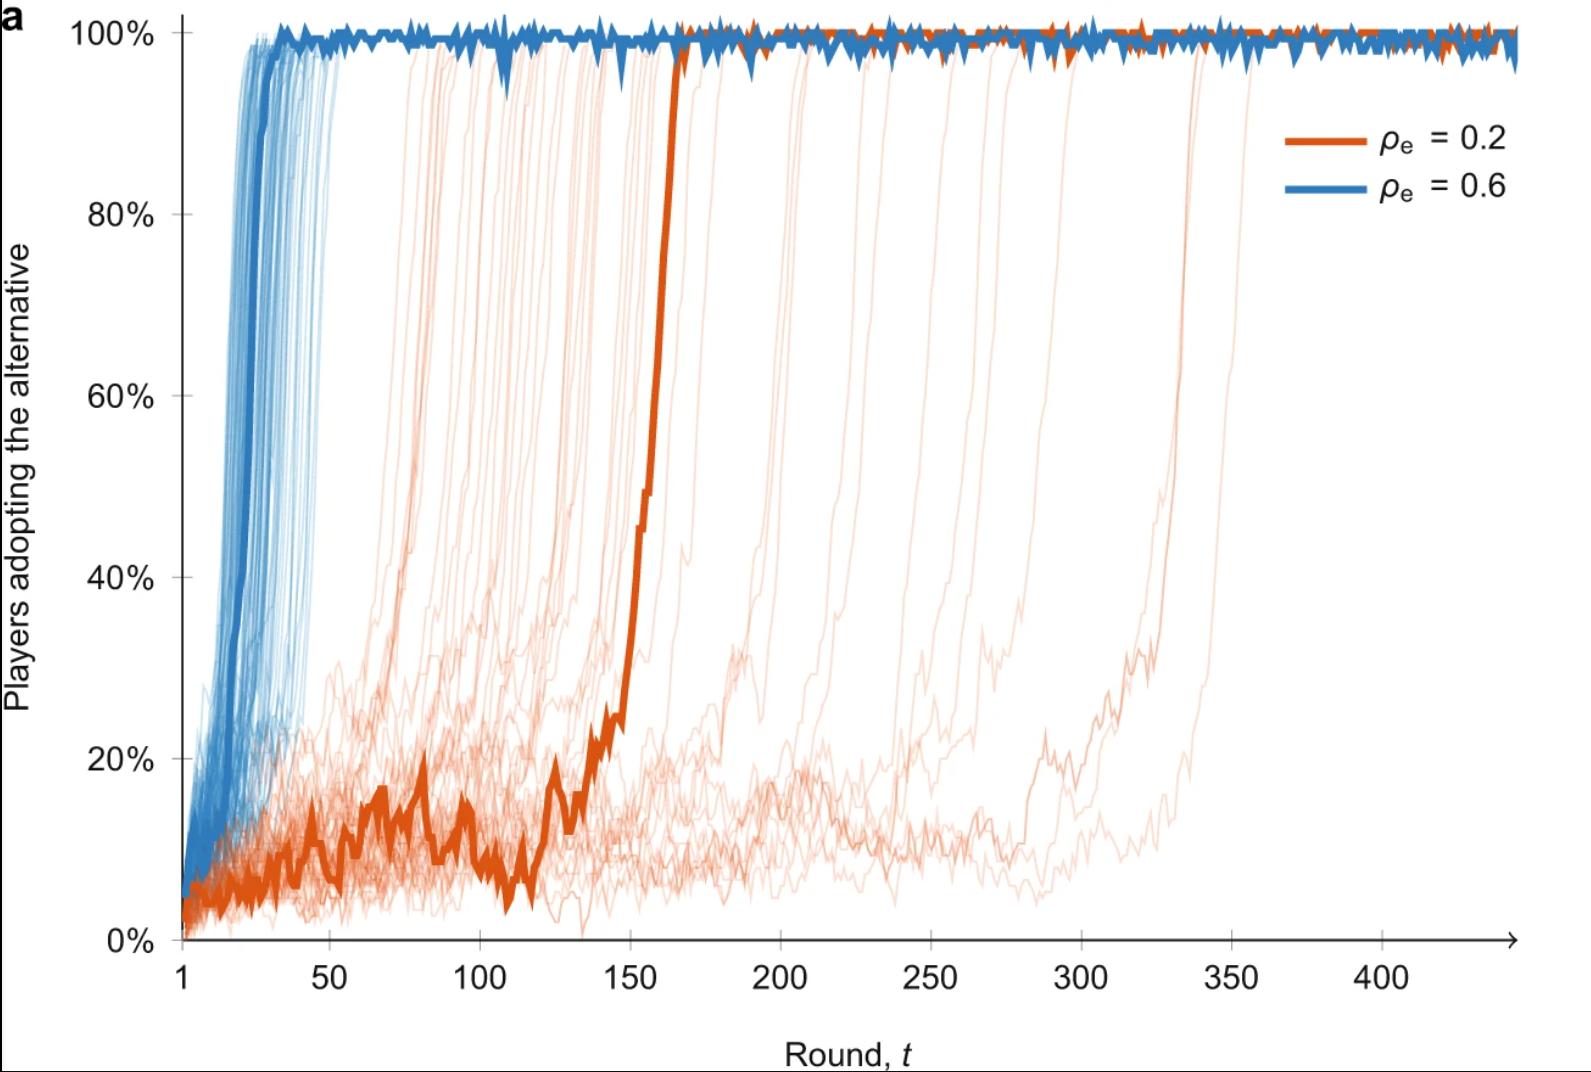
\includegraphics [width=0.7 \linewidth]{fig2.png}	     
	\end{center}
    \caption{Fig.2} \label{f1:1} 
	\end{figure}
	\end{frame}


%---------------------------------------------------------	
\section{Conclusion}
\begin{frame}
	\sectionpage
\end{frame}
	\begin{frame}
		\frametitle{A Mathematical Model Generalising the Coordination Game}
		\setlength{\parindent}{2em} 
		\addtolength{\parskip}{6pt}
		通过对实验数据的分析,惯性和趋向性在塑造社会扩散模式中发挥着关键作用。这种概括协调博弈的数学模型是一种流行的ABM扩散和决策框架,将该模型推广到其他问题中,可以研究更一般的集体决策场景,如杂交玉米种子提供更好的作物产量。
		
		目前,越来越多关于传染病的文献探索了社会扩散的个人层面动态的复杂度,该模型为进一步深入	
	    研究扩散模型中的行为机制提供了强有力的论据,这些导致了具有复杂传染特征的社会扩散,与流行病、
	    生物动力学和计算机病毒等其他传播感染过程区分开来。
    \end{frame}
	
	
%---------------------------------------------------------
\section{Reference \& Data \& Code}
	\begin{frame}
		\frametitle{Availability}
		\begin{itemize}
			\item<1-> Ye, M., Zino, L., Mlakar, Ž., Bolderdijk, J. W., Risselada, H., Fennis, B. M., & Cao, M. (2021). Collective patterns of social diffusion are shaped by individual inertia and trend-seeking. Nature communications, 12(1), 1-12.
			\item<2-> 文中所用数据和代码均来自Zenodo数据库,使用 MIT License.
			\begin{center}
				\url{https://doi.org/10.5281/zenodo.5175151}
				\url{https://github.com/lzino90/diffusion}
				\url{https://doi.org/10.1038/s41467-021-25953-1}
			\end{center}
		    \begin{center}
            \item<3-> Let's start a demo!
		    \end{center}

		\end{itemize}
	\end{frame}
	
%---------------------------------------------------------
\begin{frame}{}
	\begin{block}{}
		\centerline{\huge{\emph{\itshape{Thanks for your Listening!}}}}
	\end{block}
	\begin{center}
~\\ \small{Powered by Jie Xing with \LaTeX \\
	@jxing0831}
    \end{center}


\end{frame}
	%---------------------------------------------------------
	
	
\end{document}\\